% !Mode:: "TeX:UTF-8"
%!TEX program  = xelatex

\documentclass[bwprint]{gmcmthesis}
\usepackage[framemethod=TikZ]{mdframed}
\usepackage{longtable}
\usepackage{lineno,hyperref}
\usepackage{amsmath}
\usepackage{float}
\usepackage{graphicx}
\usepackage{subfigure}
\usepackage{caption}
\title{全国研究生数学建模竞赛论文标题}
\baominghao{4321} %参赛队号
\schoolname{XX大学}%学校名称
\membera{小米} %队员A
\memberb{向左} %队员B
\memberc{哈哈} %队员C
\begin{document}

 %生成标题
 \maketitle

 %填写摘要
\begin{abstract}
本模板是为全国研究生数学建模竞赛编写的 \LaTeX{} 模板, 旨在让大家专注于
论文的内容写作, 而不用花费过多精力在格式的定制和调整上. 本手册是相应的参考, 其
中提供了一些环境和命令可以让模板的使用更为方便. 同时需要注意, 使用者需要有一
定的 \LaTeX{} 的使用经验, 至少要会使用 ctex 宏包的一些功能, 比如调节字距或修改字体
大小等等.


\keywords{模板\quad  \LaTeX{}\quad   数学建模}
\end{abstract}

\pagestyle{plain}

%目录 不推荐加
%\tableofcontents

\section{问题重述}

\subsection{引言}

近年来,基于文本形式的在线旅游与用户生成内容愈发成为人们获取旅游信息进行攻略查询的重要信息来源。在这些信息中,有许多内容蕴含丰富的旅游相关信息,比如各文旅实体可能之间存在某种内在联系能够通过一定手段被挖掘出来,进而能够用作数据分析、营销产品设计及推荐系统等业务。因此,从众多文本数据中筛选出与文旅主题相关的信息,进而运用知识图谱手段挖掘文旅实体之间内在联系具有重要意义。

\subsection{问题的提出}

\begin{itemize}
	\item 问题一:针对附件中的微信公众号推文和游记攻略子表,根据其中每条推文或攻略与文旅的相关度进行分类,将他们分为相关或是不相关。其中与文旅相关的高频主题词可能包括:旅游,活动,交通,酒店,景区,假期,游客,农家乐等。
 
	\item 问题二:根据附件中提供的对景区、酒店等旅游产品的评价,外加游记攻略和公众号推文,对其中蕴含的旅游实体进行识别和提取。随后对上述实体构建热度评价模型,提取出其中较为热门的旅游产品实体。
 
	\item 问题三:根据表格中的OTA、UGC数据,对旅游产品进行关联度分析,找出以景区、酒店、餐饮为核心的强关联模式。并在此基础上进行可视化分析。
 
	\item 问题四:基于历史数据,分析疫情前后旅游产品变化。
\end{itemize}


% \section{模型的假设}

% \begin{itemize}
% \item 忽略实际加工误差对设计的影响;
% \item 木条与圆桌面之间的交接处缝隙较小,可忽略;
% \item 钢筋强度足够大,不弯曲;
% \item 假设地面平整。
% \end{itemize}

% \section{符号说明}

% \begin{tabular}{cc}
%  \hline
%  \makebox[0.4\textwidth][c]{符号}	&  \makebox[0.5\textwidth][c]{意义} \\ \hline
%  D	    & 木条宽度(cm) \\ \hline
%  L	    & 木板长度(cm)  \\ \hline
%  W	    & 木板宽度(cm)  \\ \hline
%  N	    & 第n根木条  \\ \hline
%  T	    & 木条根数  \\ \hline
%  H	    & 桌子高度(cm)  \\ \hline
%  R	    & 桌子半径(cm)  \\ \hline
%  R	    & 桌子直径(cm)  \\ \hline
% \end{tabular}

\section{问题分析}

\subsection{问题一分析}
利用附件中提供的公众号推文和游记攻略,本文需要构建适当模型根据其与文旅主题的相关性进行样本的有效划分。

首先,公众号推文包含标题、发表时间和正文信息。经过初步观察,推文标题和正文中都包含相与文旅相关的主题词,但其中有些正文内容收到其本身是广告或图片的形式,导致其内容体现在正文文本上与文旅主题相关程度不高。针对这类数据的预处理直接影响后续文本分类模型的好坏。

其次,游记攻略相关信息包括城市、游记标题、发布时间、出发时间、出行天数、人物、费用及正文。经过初步观察,游记攻略的标题和正文蕴含着丰富文本信息,但其中同样存在一些不相关的内容需要甄别,这也对后续的分类模型带来一定的挑战。


\subsection{问题二分析}
针对旅游产品的提取,最直观的是通过酒店、餐厅和旅游景点的评论信息进行提取,但是经过初步观察发现,在游记攻略中也蕴含丰富的文旅实体信息,如果忽略游记攻略是不妥的,在此本文考虑使用无监督学习方法对攻略中可能存在的实体信息进行提取。对旅游产品进行特征工程,最直观的为旅游产品被提及的次数,但直考虑次数不能够客观反映游客对旅游产品的满意程度,故根据文本的情感分析同样是十分必要的。


% \begin{figure}[!h]
% \centering
% 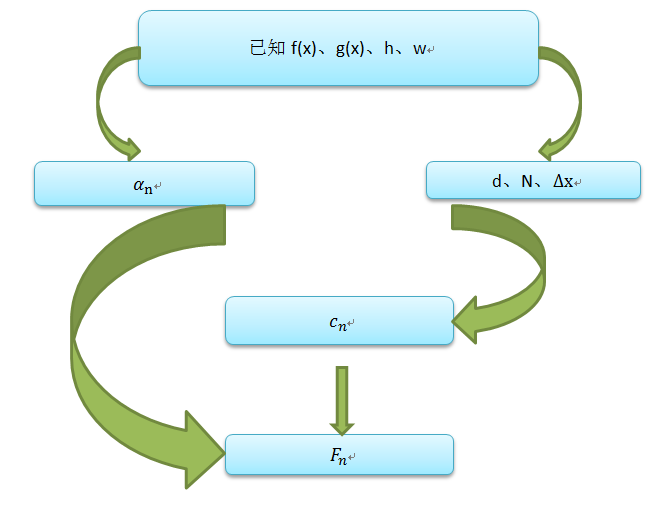
\includegraphics[width=.7\textwidth]{1.png}
% \caption{问题三流程图}
% \end{figure}

\subsection{问题三分析}
关联度构建可以考虑由公众号新闻和攻略出发进行挖掘,现有对图神经网络和知识图谱算法的研究十分热门,合理利用文本信息,挖掘其中关系,并在知识图谱火或是图神经网络中进行有效的高阶信息提取对于挖掘旅游产品之间关系十分重要。

\section{问题一建模与求解}

\subsection{数据预处理}

对于附件中给出的文本信息,由于前三问并不要求分析疫情前后文旅行业发生的变化,则首先应当将2018-2021年的数据进行合并。根据一定观察,发现公众号推文和游记的标题与正文都一定程度包含与文旅相关的内容,不能仅分析正文或是分析标题,故本文将标题与正文进行合并,用于后续的分析。

根据已经获得的文本信息,首先需要对其进行清理,将其中的数字、英文字母、特殊字符、换行符和空格等进行删除,这些信息对于基于中文的分析没有用处。对清理后的纯文本,对字段进行分词处理,方便随后进行进一步建模。

\subsection{模型构建与求解}

针对已有的文本,本文考虑构建LDA(Latent Dirichlet Allocation)主题模型实现文章与文旅相关性的划分在值得一提的是,在许多利用LDA模型进行主题分类的应用中,数据集的分布较为广泛,而考虑到本文数据集大部分与旅游是相关的,若在不引入外部数据集的情况下使用该模型,很可能分类效果不好。鉴于此,本文将LDA模型用作类似于K-means的聚类用途,根据其分类的文本特征再对文本主题进行分类。

LDA模型利用了贝叶斯的思想,将每个文本和每个主题词的先验分布均视为狄利克雷(Dirichlet)分布,其中文本词向量一致,目标是求语料库的分布。
\begin{gather}
	\theta_d \sim Dirichlet(\alpha) \\
	\beta_k \sim Dirichlet(\eta)
\end{gather}


其中随机变量$\theta_d$与$\beta_k$分别代表第$d$条文本和第$k$个主题词,$\alpha$和$\eta$分别代表分布的超参数向量,维度分别为$K$和$V$。对于第$d$条文本中的第$n$个词,根据多项分布可以得到其主题编号$z_{dn} \sim multi(\theta_d)$和词分布$w_{dn} \sim multi(\beta_{z_{dn}})$。则$(\alpha \rightarrow \theta_d \rightarrow z_d)$组成了Dirichlet-multi共轭分布。故能够得到$\theta_d$的后验分布$Dirichlet(\theta_d|\alpha + n_d)$,同样可以得到$\beta_k$的后验分布$Dirichlet(\beta_k|\eta + n_k)$。LDA模型的任务便是需要得到收敛的主题词$\beta$分布。至于LDA模型的求解,本文选用基于变分推断的EM算法。

要对文本进行基于文旅主题相关性的划分,首先要利用LDA模型进行文本主题划分。这一步本文期望得到文本数据的分类。首先本文给LDA主题模型设定了一系列主题词总共38个,包括:“旅游、活动、节庆、特产、交通、酒店、景区、景点、文创、文化、乡村旅游、民宿、假日、假期、游客、采摘、赏花、春游、踏青、康养、公园、滨海游、度假、农家乐、剧本杀、旅行、徒步、工业旅游、线路、自驾游、 团队游、攻略、游记、包车、玻璃栈道、游艇、高尔夫、温泉”。随后,运用LDA主题模型得到每条文本分属$K$个分类的概率,并统计了每个类中的单词的出现频率,并提取其中最常出现的$D$个词汇, 上述$D$,$K$为模型超参数。

对LDA主题模型分得的$K$个类别,本文将其中每类的高频词汇提出,分别将每类对应的高频词汇与文旅相关主题词进行匹配,匹配度达到一定阈值$\gamma$则认定该类属于与文旅主题相关,否则为不相关,值得一提的是阈值$\gamma$在本文中也为超参数。此外本文通过pyLDAvid和pyLDAvis对主题进行可视化。

经过多次实验,发现将公众号推文分为6类,游记攻略分为5类的时候分类效果较好,图\ref{lda_fenlei}给出了两个文本数据经过LDA主题模型分类后的可视化结果。

\begin{figure}[H]
    \centering
    \subfigure[微信公众号推文]{
        \label{newslda}
        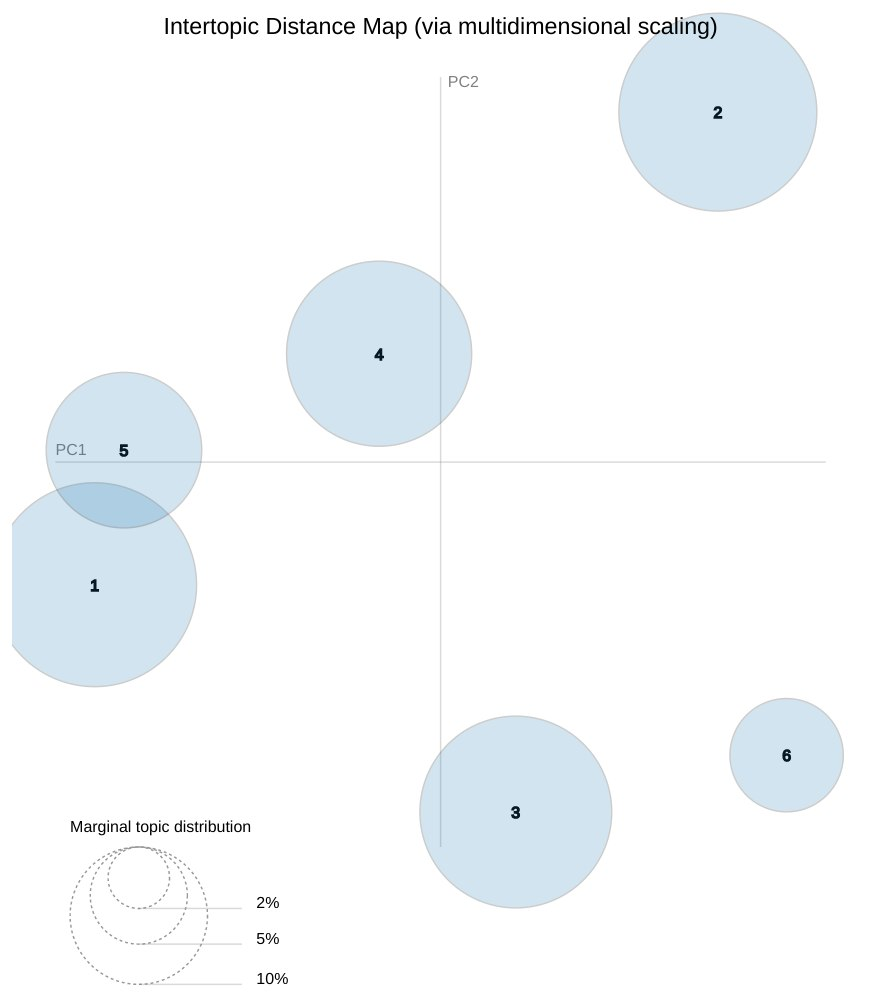
\includegraphics[width=0.45\textwidth]{figures/news_lda.png}
    }
    \hspace{0in}
    \subfigure[游记攻略]{
        \label{travellda}
        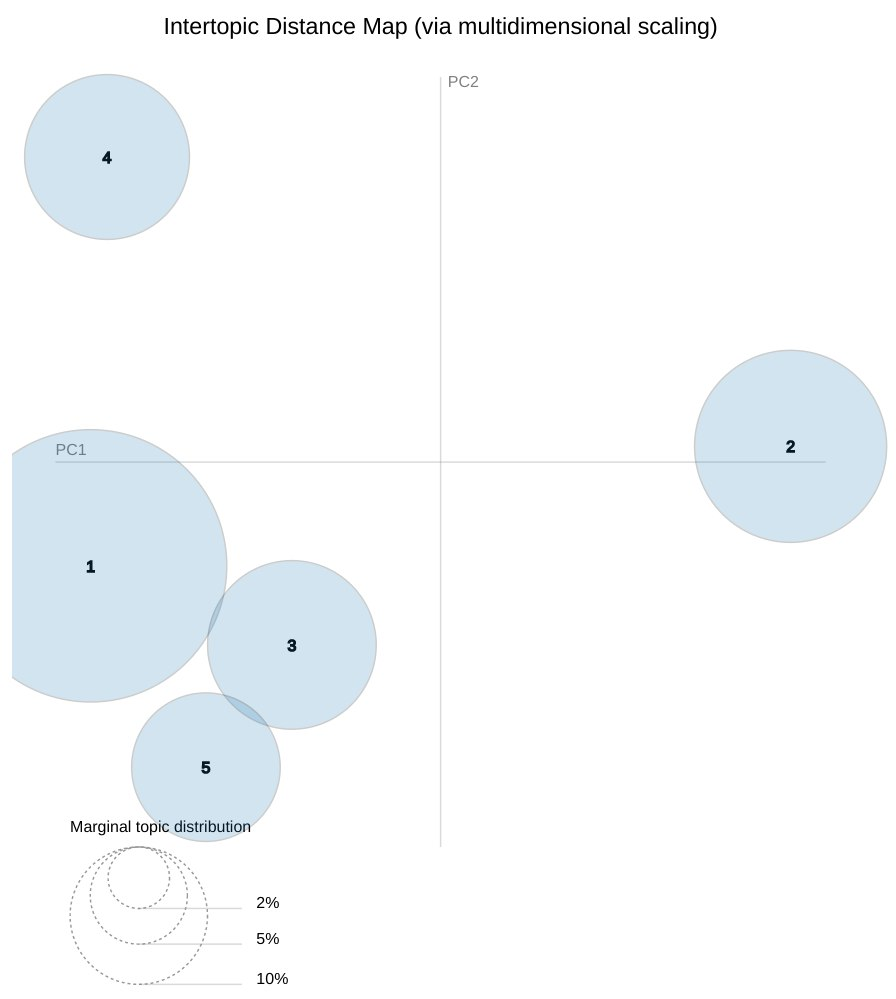
\includegraphics[width=0.45\textwidth]{figures/travel_lda.png}
    }
    \caption{基于LDA模型的文本主题分类}
    \label{lda_fenlei}
\end{figure}

为了验证分类后每个分类与文旅主题词库的匹配程度,本文首先需要对每类文本中的高频词汇进行统计。

对于公众号推文,本文发现,在超参数$K=6$,$\gamma=0$的时候,分类的效果较为理想,经过初步可视化,以其中四个分类的高频词为例,如图\ref{news1}、\ref{news2}、\ref{news3}及\ref{news4}所示:


\begin{figure}[H]
	\centering
	\begin{minipage}{0.49\linewidth}
		\centering
		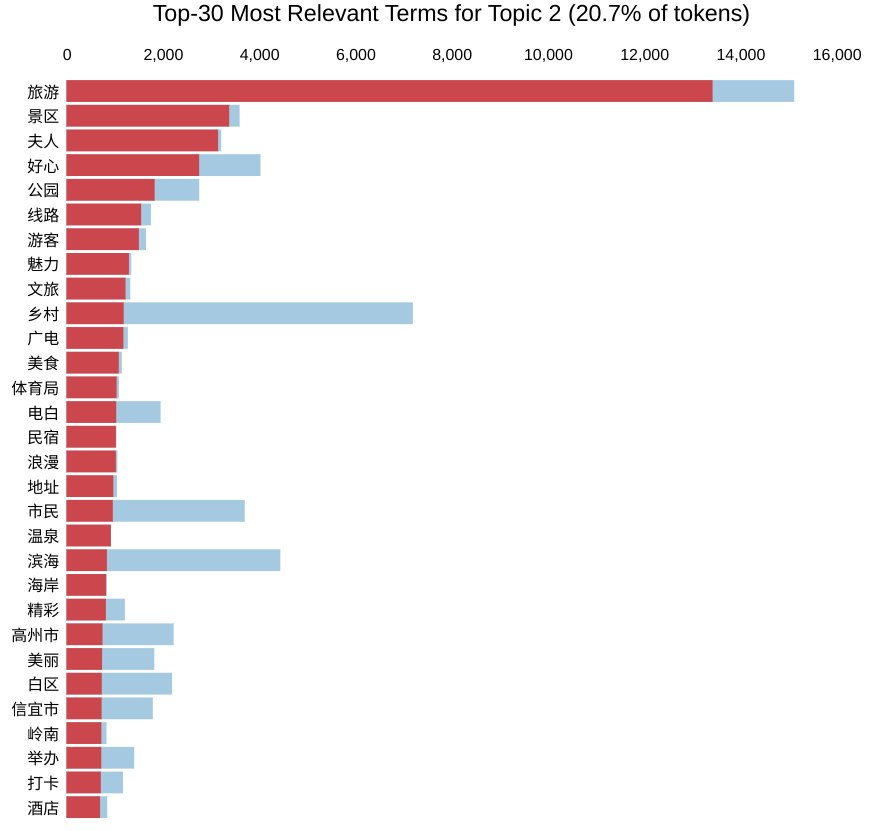
\includegraphics[width=0.9\linewidth]{figures/news1.png}
		\caption{分类2}
		\label{news1}%文中引用该图片代号
	\end{minipage}
	\begin{minipage}{0.49\linewidth}
		\centering
		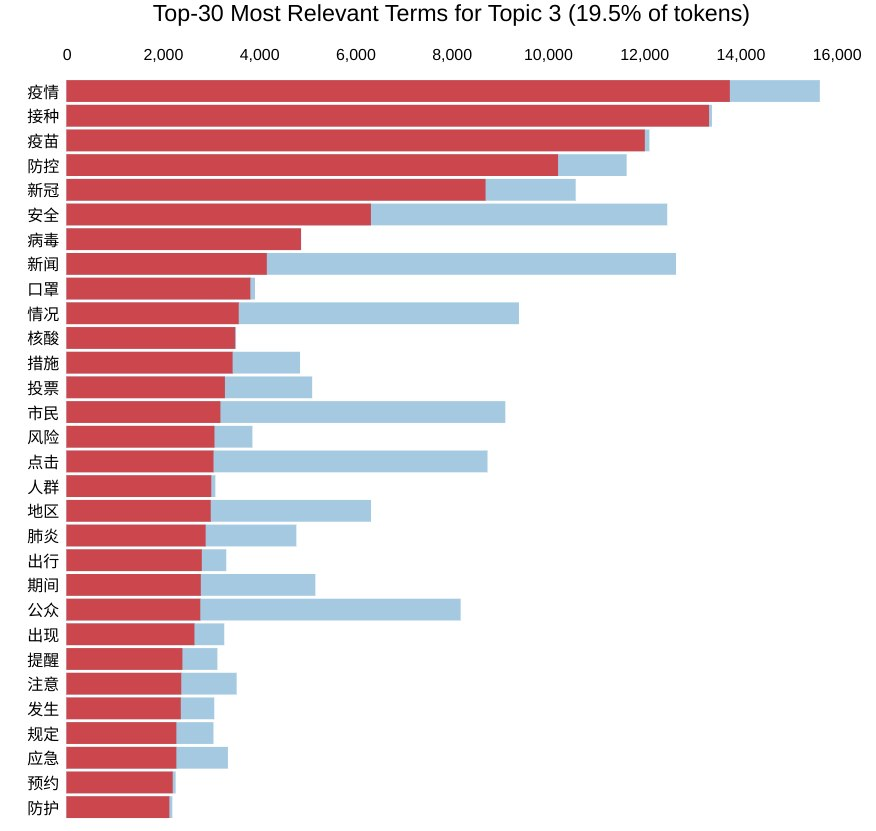
\includegraphics[width=0.9\linewidth]{figures/news2.png}
		\caption{分类3}
		\label{news2}%文中引用该图片代号
	\end{minipage}
	%\qquad
	%让图片换行,
	
	\begin{minipage}{0.49\linewidth}
		\centering
		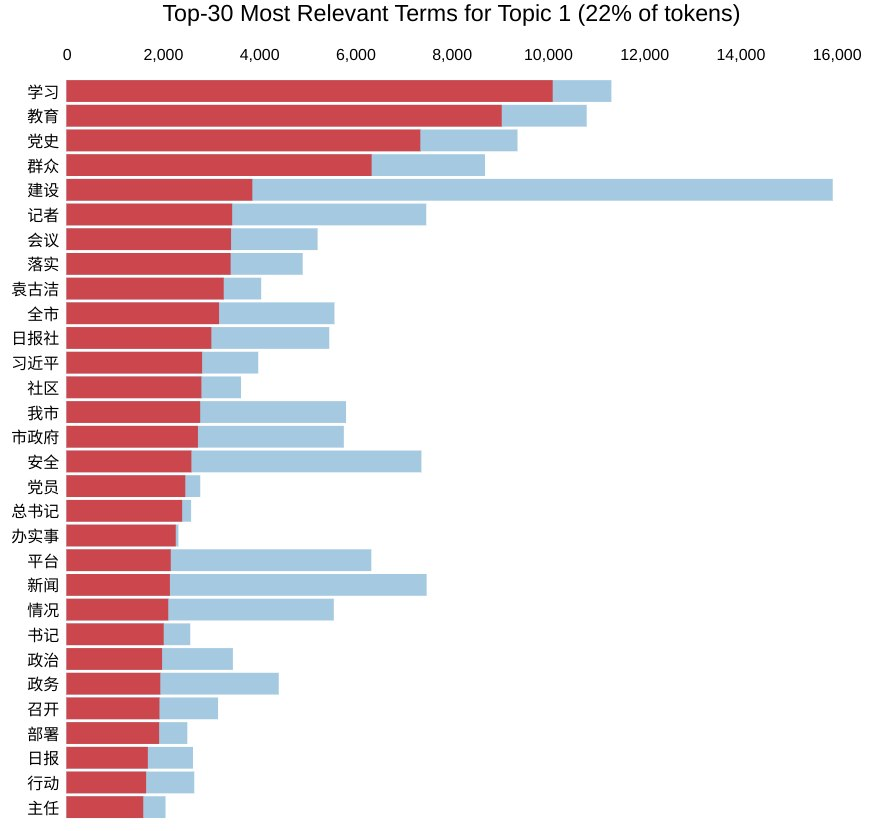
\includegraphics[width=0.9\linewidth]{figures/news3.png}
		\caption{分类1}
		\label{news3}%文中引用该图片代号
	\end{minipage}
	\begin{minipage}{0.49\linewidth}
		\centering
		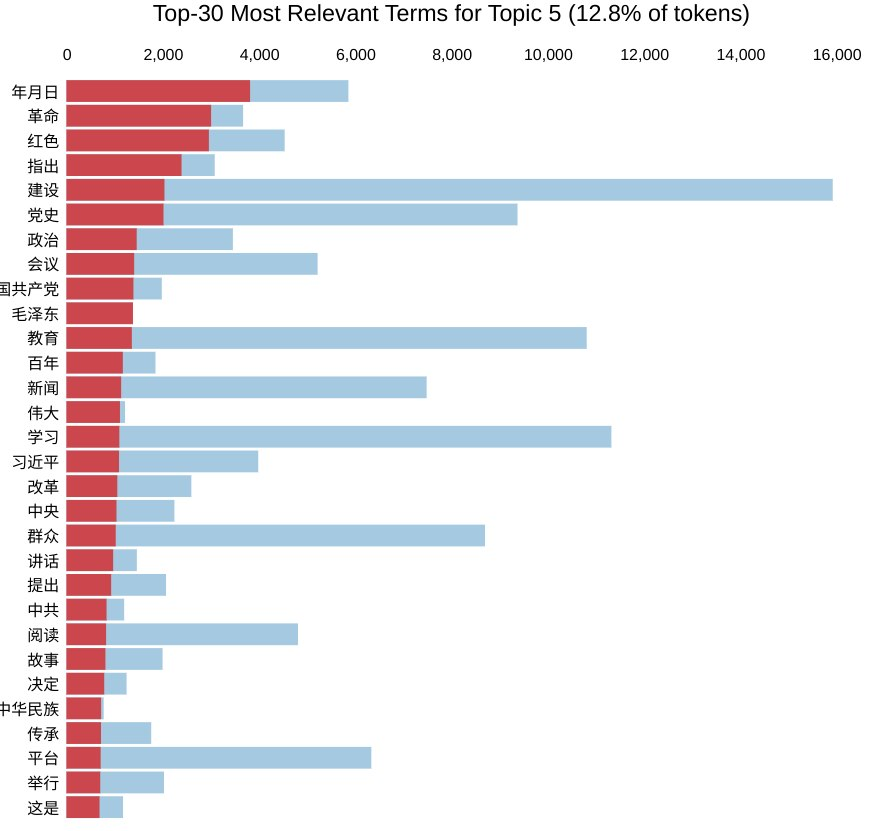
\includegraphics[width=0.9\linewidth]{figures/news4.png}
		\caption{分类5}
		\label{news4}%文中引用该图片代号
	\end{minipage}
\end{figure}

经过初步观察,基于LDA的建模是有效的,图\ref{news1}中展示的分类2的公众号推文高频词汇,其中大多都与文旅主题相关,而图\ref{news2}中显示分类3中的推文基本与疫情相关,图\ref{news2}中显示分类1和5中的推文则与党建、政府工作相关性较大。

对于旅游攻略,本文发现,在超参数$K=5$,$\gamma=0$的时候,分类的效果较为理想,经过初步可视化,以其中两个分类的高频词为例,如图\ref{travel_cipin}所示:

\begin{figure}[H]
    \centering
    \subfigure[分类1]{
        \label{travel1}
        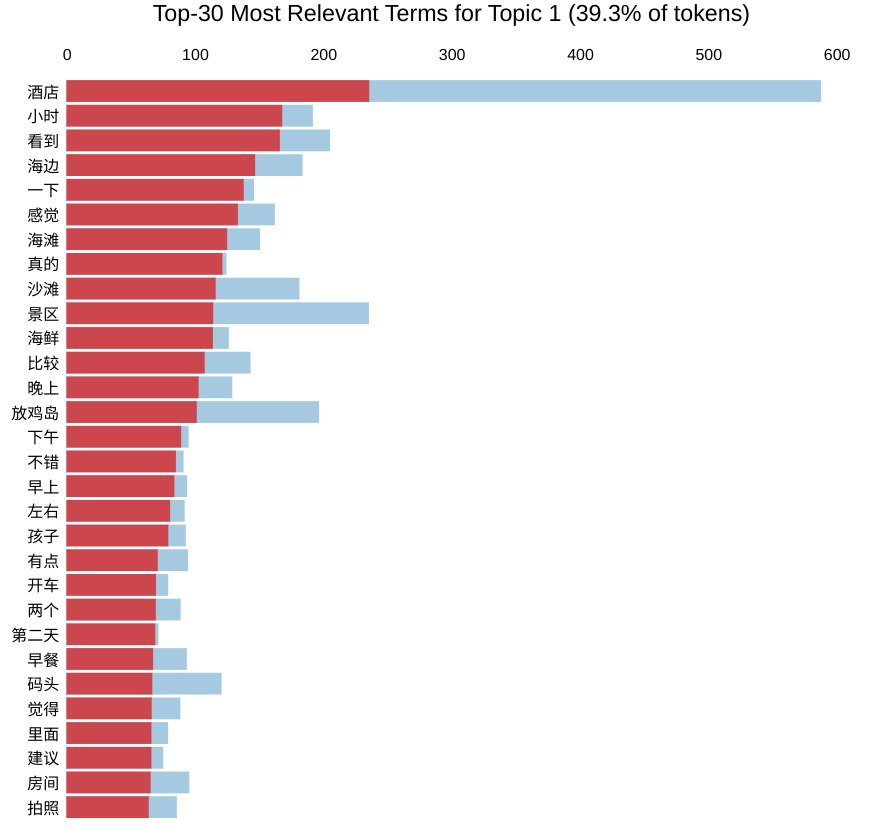
\includegraphics[width=0.45\textwidth]{figures/travel1.png}
    }
    \hspace{0in}
    \subfigure[分类2]{
        \label{travel2}
        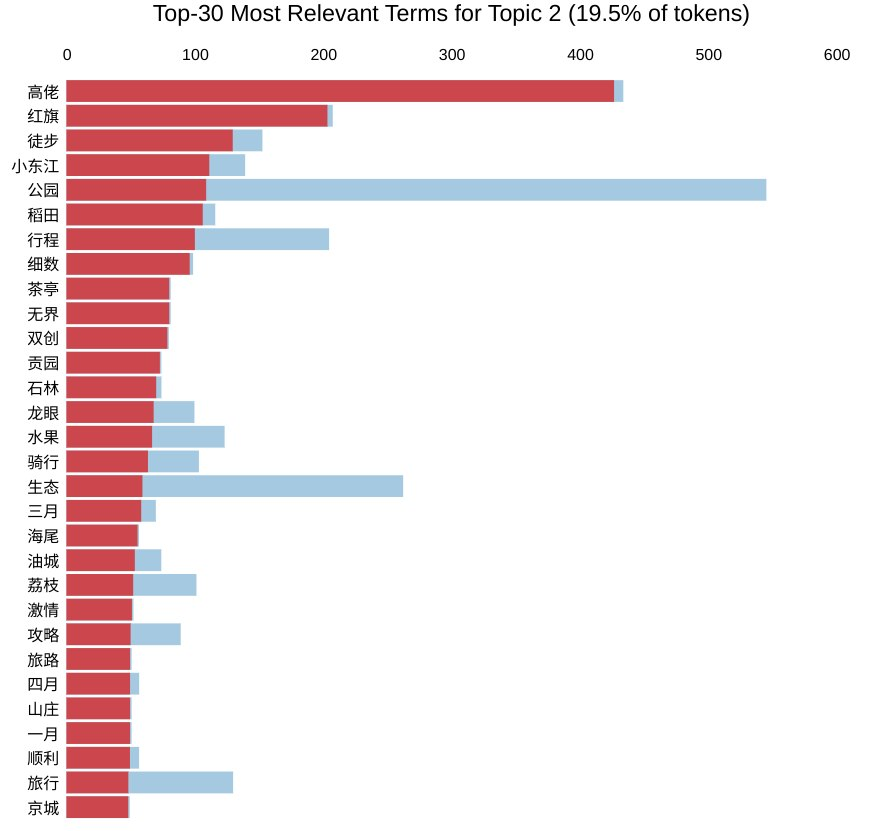
\includegraphics[width=0.45\textwidth]{figures/travel2.png}
    }
    \caption{基于LDA模型的旅游攻略词频分析}
    \label{travel_cipin}
\end{figure}

通过图\ref{travel_cipin}能够看出,LDA主题模型的分类对于旅游攻略文本同样是有效的,文旅相关的文本与党建、团建等无关主题的文本被有效提取了出来。根据上述LDA主题模型的分类结果分析,能够看出该模型对于文本的分类还是较为清晰的,至于文旅主题相关性的判别,本文根据每类文本中高频词与主题词库中高频词的匹配程度对文本进行相关性预测。根据阈值$\gamma$,本文首先选取LDA主题分类中与文旅主题相关的类,该类下的所有样本都被视作与文旅主题相关。相应的,若主题匪类的高频词与主题词库的匹配程度如果低于阈值$\gamma$,则该类中的所有样本都被视作与文旅主题无关。

下表给出了微信公众号推文和游记攻略与文旅主题相关性的判断:

\begin{center}
    \begin{longtable}{c|c|c}
      \caption{微信公众号推文及游记攻略与文旅主题相关性预测}
      \label{wx_yj_related}\\
        \hline
        \textbf{文本类别} & \textbf{相关性} & \textbf{ID(由小到大排序)} \\
        \hline
          公众号推文 & \begin{tabular}[c]{@{}c@{}}
            相关 \\ 不相关 
          \end{tabular} 
          & \begin{tabular}[c]{@{}l@{}}
            1001,1004,1006,1008,……,7267,7269,7281,7284 \\ 1002,1003,1005,1007,……,7282,7283,7285,7286
          \end{tabular} \\
		  游记攻略 & \begin{tabular}[c]{@{}c@{}}
            相关 \\ 不相关 
          \end{tabular} 
          & \begin{tabular}[c]{@{}l@{}}
            1001,1003,1004,1006,……,1291,1292,1293,1294 \\ 1002,1005,1007,1020,……,1211,1251,1254,1266
          \end{tabular} \\
        \hline
    \end{longtable}
    \end{center}

\section{问题二建模与求解}

\subsection{模型的构建与求解}

\section{问题三建模与求解}

\subsection{图卷积神经网络}

图神经网络(GNN)是近年来十分热门的研究课题。在图神经网络中,实体被视作节点,而实体之间的联系被视作连接节点的边。通过利用神经网络优秀的表现能力,结合知识图谱的范式,图神经网络能够充分提取有连接的节点之间的高阶连接信息,进而能够完成一系列如:节点分类、连接预测等任务。

图卷积神经网络(GCN)作为图神经网络的一种,的得名来源于卷积神经网络(CNN)的思想。卷积神经网络是在二维平面对节点做卷积运算,而图神经网络将这一运算拓展至三维空间。GNN中计算最终输出过程中起主要作用的是特征信息聚合与传递。信息传递表现的是节点信息在不同的神经网络层之间的计算,而信息聚合表示的是不同神经网络层之间的节点、连接信息的聚合计算。在信息传递过程中,节点$v$接收来自于每个与其相邻的节点$u$的信息$m_{u}^{(l)}$为:
\begin{equation}
  m_{u}^{(l)} = \frac{W^{(l)}}{|N(v)|}(h_u^{(l-1)}), \ u \in \{N(v) \cup v\}
\end{equation}

其中$W^{(l)}$为可训练的权重参数,$|N(v)|$的引入是为了防止表征在传递与聚合的过程中发生信息在数量级上的变化。

而节点$v$在第$l$层卷积层其自身的表征$h_v^{l}$为:
\begin{gather}
	h_{v}^{(l)} = AGG^{(l)}(\{m_u^{(l)}, u \in N(v), m_v^{(l)}\}), \ u \in \{N(v) \cup v\} \\ 
	= \sigma(\sum \frac{W^{(l)}}{|N(v)|}(h_u^{(l-1)}), \ u \in \{N(v) \cup v\})
\end{gather}

其中$\sigma$为激活函数,$AGG^{(l)}$表示的是聚合函数,在GCN中该函数为和函数。在$l$层神经网络层的传递与聚合后,节点就能够获得其$l-1$阶近邻的信息。

\subsection{模型的构建与求解}

本文基于图卷积神经网络(GCN)进行节点间的链路预测。首先,本文根据前文的Bert模型,对每个实体提取了一个768维度的表征,用于刻画该实体的内在特征。随后,根据文本在同一篇微信公众号推文或游记攻略中的同时出现情况,则本文认为这两个实体是具备关联的。本文在这里将已有的768维节点表征作为每个节点的初始表征,用于随后的表征的传递与聚合。

\section{问题四建模与求解}

新冠疫情对于旅游行业有重大的影响,最直观的就是短途旅行的增多。显然疫情对于旅游产品实体和实体时间的关联都存在一定影响。

首先为了分析疫情对于旅游产品实体自身的影响,本文对提取得到的节点实体在疫情前后的情感的的得分及热度分别进行评估。

%参考文献   手工录入
%\begin{thebibliography}{9}%宽度9
% \bibitem{bib:one} ....
% \bibitem{bib:two} ....
%\end{thebibliography}

%采用bibtex方案
\cite{wright_latex3_2009}

\bibliographystyle{gmcm}
\bibliography{example}


% \newpage
% %附录
% \appendix
% %\setcounter{page}{1} %如果需要可以自行重置页码。
% \section{我的 MATLAB 源程序}
% \begin{lstlisting}[language=Matlab]%设置不同语言即可。
% kk=2;[mdd,ndd]=size(dd);
% while ~isempty(V)
% [tmpd,j]=min(W(i,V));tmpj=V(j);
% for k=2:ndd
% [tmp1,jj]=min(dd(1,k)+W(dd(2,k),V));
% tmp2=V(jj);tt(k-1,:)=[tmp1,tmp2,jj];
% end
% tmp=[tmpd,tmpj,j;tt];[tmp3,tmp4]=min(tmp(:,1));
% if tmp3==tmpd, ss(1:2,kk)=[i;tmp(tmp4,2)];
% else,tmp5=find(ss(:,tmp4)~=0);tmp6=length(tmp5);
% if dd(2,tmp4)==ss(tmp6,tmp4)
% ss(1:tmp6+1,kk)=[ss(tmp5,tmp4);tmp(tmp4,2)];
% else, ss(1:3,kk)=[i;dd(2,tmp4);tmp(tmp4,2)];
% end;end
% dd=[dd,[tmp3;tmp(tmp4,2)]];V(tmp(tmp4,3))=[];
% [mdd,ndd]=size(dd);kk=kk+1;
% end; S=ss; D=dd(1,:);


%  \end{lstlisting}


\end{document} 